\subsection{Gas de Fermi}{\label{sec:intro_fermi_gas}}

En los sistemas cuánticos, la indistinguibilidad de las partículas juega un rol esencial.
Esta indistinguibilidad obliga a todos los autoestados $\ket{\Psi}$ del sistema a ser autoestados del operador permutación de 2 partículas $\hat{P}_{ij}$ (permuta la $i$-esima con la $j$-esima), cuyos únicos autovalores son $\pm 1$.
De esta manera, se asegura la invarianza de los observables ante $\hat{P}_{ij}$
\[\bra{\Psi'}\hat{A}\ket{\Psi'} = \bra{\Psi}\hat{P}^\dagger\hat{A}\hat{P}\ket{\Psi} = (\bra{\Psi}\pm)\hat{A}(\pm\ket{\Psi}) = \bra{\Psi}\hat{A}\ket{\Psi}\]

Se llaman \textit{bosones} a las partículas cuyas funciones de onda tienen autovalor positivo ante cualquier permutación de 2 partículas (simétricas $\hat{P}_{ij}\ket{\Psi} = \ket{\Psi}$) y \textit{fermiones} a aquellas con autovalor negativo (antisimétricas $\hat{P}_{ij}\ket{\Psi} = -\ket{\Psi}$).
De esta propiedad de los fermiones surge el principio de exclusión de Pauli, que prohíbe la ocupación de un mismo estado por más de un fermion.
De otra forma, sería imposible lograr que la función de onda sea antisimétrica, dado que si tuviésemos dos partículas $i$ y $j$ en el mismo estado, la permutación $\hat{P}_{ij}$ mantendría
$\ket{\Psi}$ invariante en lugar de cambiar su signo.

Según el teorema de spin-estadística de Dirac, los fermiones poseen spin semi-entero $s=l+1/2$, razón por la que los nucleones (protones y neutrones) y los electrones son fermiones.
La exclusión de Pauli es fundamental a la hora de comprender la dinámica de fermiones a bajas temperaturas.
Dada esta exclusión, aún a temperatura cero resulta imposible que todos los fermiones condensen a sus autoestados (de única partícula) de menor energía. 
Esto hace que los distintos niveles de energía se ``llenen'' uno a uno, lo cual inevitablemente genera sistemas con mayor energía total.
Gracias a esto puede explicarse desde la conducción eléctrica en metales\cite[pp. 247]{BOOK:PATHRIA} hasta la \textit{presión de degeneración} 
(presión no nula a temperatura cero) que evita el colapso de las enanas blancas \cite[pp. 259]{BOOK:PATHRIA}.

El sistema de fermiones no interactuantes es el más simple, cuya estadística es bien conocida, siendo su función de partición gran canónica y ocupación media\cite[pp. 231]{BOOK:PATHRIA}
\begin{equation}
 \frac{PV}{k_BT} \equiv \log Z = \sum_\varepsilon \log(1+ze^{-\beta\varepsilon})
\end{equation}
\begin{equation}
 N = \sum_\varepsilon \langle n_\varepsilon\rangle = \sum_\varepsilon \frac{1}{z^{-1}e^{\beta\varepsilon}+1}
\end{equation}
con $z=e^{\beta\mu}$ la fugacidad, $\beta=1/k_BT$ y $\mu$ el potencial químico del sistema.
Los niveles de energía de una partícula $\varepsilon=p^2/2m$ están discretizados y dependen del volumen $V$, con $\Delta\varepsilon\sim V^{-1/3}$.

En el límite termodinámico ($V\to\infty$), la diferencia entre energías $\Delta\varepsilon\to 0$ y podemos transformar la sumatoria en una integral en el espacio de fases.
Realizando las integrales triviales, resulta
\begin{equation}{\label{eq:Z_cont}}
 \frac{PV}{k_BT} \equiv \log Z = \frac{4\pi V}{h^3} \int_0^\infty \log(1+ze^{-\beta p^2/2m})p^2dp = \frac{gV}{\lambda^3}f_{5/2}(z)
\end{equation}
\begin{equation}{\label{eq:N_cont}}
 N = \frac{4\pi V}{h^3} \int_0^\infty \frac{1}{z^{-1}e^{\beta p^2/2m}+1} p^2dp = \frac{gV}{\lambda^3}f_{3/2}(z)
\end{equation}
donde $g$ es un factor de degeneración asociado a grados de libertad internos (spin, por ejemplo) y  $\lambda$ es la longitud de onda térmica
\[ \lambda = \sqrt{ \frac{2\pi\hbar^2}{mk_BT} } \]
y las $f_\nu(z)$ son las funciones de Fermi-Dirac definidas según
\[ f_\nu(z) = \frac{1}{\Gamma(\nu)}\int_0^\infty \frac{x^{\nu-1}}{z^{-1}e^x+1} = \sum_{l=1}^\infty (-1)^{l+1}\frac{z^l}{l^\nu}\]

Para un sistema de número de partículas, volumen y temperatura constante (o NVT), debemos obtener la fugacidad $z$ invirtiendo \eqref{eq:N_cont}, lo que introduce el problema de computar las funciones de Fermi-Dirac $f_\nu(z)$.
Al ser series alternadas, la convergencia de las sumas parciales es muy lenta y debemos recurrir a otros métodos, que detallamos en el Apéndice \ref{ap:func_fermi}.
Independientemente de esto, puede verse que obtendremos un $\mu(N/V,T) = \mu(\rho, T)$, cuya dependencia en $\rho$ en lugar de $N$ y $V$ por separado es razonable al ser $\mu$ una magnitud intensiva.

En particular, podemos ver en \eqref{eq:N_cont} la aparición del producto $\lambda^3\rho \sim T^{-3/2}\rho$ a la hora de despejar $f_{3/2}(z)$, que resulta central para las propiedades del sistema.
Para $\lambda^3\rho \sim T^{-3/2}\rho\to0$ tenemos $f_{3/2}(z)$ pequeño, por lo que a primer orden tenemos $f_{3/2}(z)\approx z\to 0$.
Reemplazando en \eqref{eq:Z_cont} y \eqref{eq:N_cont} y dividiendo ambas ecuaciones, tenemos 
\[ \frac{PV}{Nk_BT} = \frac{f_{5/2}(z)}{f_{3/2}(z)} \approx 1 \]
que resulta la ecuación de estado de un gas ideal clásico, lo cual esperamos que ocurra a alta temperatura (o baja densidad).
Por lo tanto, la noción de alta temperatura (o baja densidad) viene dada por el valor del producto $\lambda^3\rho$, tal que $T\to\infty$ resulta equivalente a $\rho\to0$.
El caso opuesto $\lambda^3\rho\to\infty$ corresponde a baja temperatura (o alta densidad), donde las propiedades cuánticas son más apreciables.

El integrando de \eqref{eq:N_cont} puede considerarse como la densidad de partículas $f(p)$ con impulso de módulo $p$.
Esta distribución de impulsos es característica de un gas de fermiones isótropo y homogéneo.
Equivalentemente, podríamos analizar la distribución de energías cinéticas $\varepsilon=p^2/2m$ mediante un cambio de variables sobre la integral de \eqref{eq:N_cont}
($d\varepsilon = pdp/m = \sqrt{2m\varepsilon}dp/m$)

\[ N = \frac{4\pi V}{h^3} \int_0^\infty \frac{1}{e^{\beta(\varepsilon-\mu)}+1} 2m\varepsilon\frac{m}{\sqrt{2m\varepsilon}}d\varepsilon =
\int_0^\infty \frac{4\pi V\sqrt{2m^3\varepsilon}}{h^3}\frac{1}{e^{\beta(\varepsilon-\mu)}+1} d\varepsilon\]

Por lo tanto, la distribución de impulsos toma la forma
\begin{equation}{\label{eq:dist_FD}}
 f_{FD}(\varepsilon) = \frac{4\pi V \sqrt{2m^3\varepsilon}}{h^3}\frac{1}{e^{\beta(\varepsilon-\mu)}+1} = \frac{G(\varepsilon)}{e^{\beta(\varepsilon-\mu)}+1}
 %= N\frac{V}{\lambda^3}\sqrt{\frac{4\beta^3\varepsilon}{\pi}}\frac{1}{e^{\beta(\varepsilon-\mu)}+1}
\end{equation}
donde $G(\varepsilon)$ es la degeneración de estados con energía $\varepsilon$ y asumimos $\mu=\mu(\rho,T)$.

En el límite de altas temperaturas (o baja densidad), esperamos que el sistema pierda sus propiedades cuánticas y recuperemos el gas clásico, donde las partículas
se vuelven distinguibles nuevamente.
Además de recuperar la ecuación de estado del gas ideal, esperamos que en el límite $\lambda^3\rho\to0$, la distribución de energías cinéticas tienda a la de un gas clásico.
Para un sistema de partículas clásico interactuando con potenciales dependientes de la posición $U(\mathbf{q}_1,..,\mathbf{q}_N)$, la distribución de energías cinéticas resulta
corresponde a la de Boltzmann (ver \textbf{Apéndice \ref{ap:boltzmann}}).
\begin{equation}{\label{eq:dist_MB}}
 f_{MB}(\varepsilon) = N\sqrt{\frac{4\beta^3\varepsilon}{\pi}}e^{-\beta\varepsilon}
\end{equation}



\subsection{Potencial de Pauli}{\label{sec:intro_pauli}}

Dado que la distribución \eqref{eq:dist_MB} es común a todo sistema de partículas distinguibles (o clásicas) cuyos Hamiltonianos dependan del momento únicamente
a través de la energía cinética (ver  \textbf{Apéndice \ref{ap:boltzmann}})
\[ H(\mathbf{q}_1,..,\mathbf{q}_N,\mathbf{p}_1,..,\mathbf{p}_N) = \sum_i \frac{p_i^2}{2m} + U(\mathbf{q}_1,..,\mathbf{q}_N)\]
la única forma de obtener una distribución de energías distinta con partículas distinguibles es introduciendo potenciales dependientes de momentos al Hamiltoniano.

Esto puede hacerse de varias maneras, pero en particular buscamos una cuya distribución resulte similar a \eqref{eq:dist_FD}.
Para esto, necesitamos poder expresar la noción de Exclusión de Pauli con un potencial de interacción de dos partículas $V(\mathbf{q}_1,..,\mathbf{q}_N;\mathbf{p}_1,..,\mathbf{p}_N)$.
Esto lo haremos imponiendo un ``costo energético'' cada vez que 2 partículas tengan un $\mathbf{q}, \mathbf{p}$ similar.
Buscamos lograr esto agregando al Hamiltoniano un potencial de interacción de 2 partículas que llamaremos \textit{potencial de Pauli} definido según

\begin{equation}{\label{eq:def_int_pauli}}
 V_P(\mathbf{q}_1,\mathbf{q}_2;\mathbf{p}_1,\mathbf{p}_2) = De^{-\frac{1}{2}\left( \frac{|\mathbf{q}_1-\mathbf{q}_2|^2}{q_o^2} +\frac{|\mathbf{p}_1-\mathbf{p}_2|^2}{p_o^2} \right)}
\end{equation}
donde surge la noción de distancia reducida en el espacio de fases $s^2 = \frac{|\mathbf{q}_1-\mathbf{q}_2|^2}{q_o^2} +\frac{|\mathbf{p}_1-\mathbf{p}_2|^2}{p_o^2}$.

Podemos visualizar los parámetros $q_o$ y $p_o$ como los ejes de un elipsoide en $\mathbb{R}^6$ (el espacio de fases) donde $s^2 \leq 1$ y el costo energético de cualquier partícula
que ingrese es $\approx D$.
A energías (o temperaturas) bajas, este costo energético puede ser suficientemente alto como para evitar la superposición de estos elipsoides en el espacio de fases, generando efectivamente
la noción de exclusión de Pauli: dos partículas no pueden estar en el mismo estado $(\mathbf{q}, \mathbf{p})$.
Es importante notar que este potencial no es de núcleo duro y, por lo tanto, es posible que dos partículas se superpongan para energías suficientemente altas donde $D$ sea despreciable.
Esto es deseable dado que para energías (o temperaturas) altas esperamos recuperar el gas clásico de Maxwell-Boltzmann al desaparecer $V_P$.

Este potencial fue inicialmente propuesto por Dorso \cite{Dorso1987, Dorso1988, Dorso1993} y utilizado en múltiples trabajos desde entonces\cite{Maruyama2012, Taruna2008}.
Los parámetros $D$, $q_o$ y $p_o$ varían en cada trabajo, adaptándose según la característica que se busque analizar.
Existen formulaciones alternativas como la de Piekarewicz \cite{Taruna2008} que proponen otra forma de abordar la exclusión de Pauli; exclusión en $q$ y en $p$ independientemente.

La dependencia del potencial con el impulso trae aparejada una serie de dificultades a la hora de hacer simulaciones de Dinámica Molecular.
Más allá de la inmediata dificultad para evolucionar el sistema (que analizaremos en la sección que sigue), surge la dificultad de definir algunas magnitudes termodinámicas del
sistema como la presión $P$ y la temperatura $T$.
Para un potencial dependiente de momentos, la temperatura $T$ no resulta la energía cinética media del sistema.
El teorema del virial (ver Apéndice \ref{ap:teo_virial}) nos permite calcular ambas magnitudes según
\begin{equation}{\label{eq:virial_T}}
k_B T =  \frac{1}{3N}\left<\sum_{i=1}^{3N} \dot{q}_ip_i \right>
=  \frac{1}{3N}\left<\sum_{i=1}^{3N} \frac{p_i^2}{m} \right> - \frac{1}{3V}\left< \sum_{i=1}^{3N}\sum_{j\neq i} \dpart{V_{ij}^{(P)}}{p_i}p_i \right>
\end{equation}

\begin{equation}{\label{eq:virial_P}}
P = \frac{1}{3V}\left< \sum_{i=1}^{3N} \dot{q}_ip_i + \dot{p}_iq_i \right>
= \frac{1}{3V}\left< \sum_{i=1}^{3N} \frac{p_i^2}{m} \right> - \frac{1}{3V}\left< \sum_{i=1}^{3N}\sum_{j\neq i} \dpart{V_{ij}^{(P)}}{q_i}q_i+\dpart{V_{ij}^{(P)}}{p_i}p_i \right>
\end{equation}

\subsection{Integración simpléctica de sistemas hamiltonianos}

La evolución de las $d$ coordenadas generalizadas $q \equiv (q_1,..,q_d)\in\mathbb{R}^{d}$ y $p \equiv (p_1,..,p_d)\in\mathbb{R}^{d}$ está definida por el Hamiltoniano
$H(q_1,..,q_d,p_1,..,p_d) \equiv H(q,p)$  a través de las ecuaciones de Hamilton
\begin{align*}
 \dot{q} &= \dpart{H}{p}(q,p) \\
 \dot{p} &= -\dpart{H}{q}(q,p)
\end{align*}
que podemos compactar definiendo $y=(p,q)\in\mathbb{R}^{2d}$ y la matriz $J = \begin{pmatrix}0 & \mathbb{I} \\-\mathbb{I} & 0\end{pmatrix}$ (con la propiedad $J^{-1} = J^T = -J$)
\begin{equation}{\label{eq:ec_hamilton}}
 \dot{y} = J^{-1}\nabla H(y)
\end{equation}

Para un Hamiltoniano que no depende explícitamente del tiempo, la ecuación de evolución \eqref{eq:ec_hamilton} asegura la conservación de $H(q,p)$ en el tiempo
\[ \frac{dH}{dt}(y) = \nabla H(y)\cdot \dot{y} = \nabla H(y)^T J^{-1}\nabla H(y) = 0\]
donde usamos que $(a,b)J^{-1}\begin{pmatrix}a\\b\end{pmatrix} = (b, -a)\begin{pmatrix}a\\b\end{pmatrix} = 0$ $\forall a,b$.
Esto no es más que la conocida conservación de la energía.

\subsubsection{Transformaciones simplécticas}{\label{sec:trans_simp}}

Además de conservar la energía, los sistemas hamiltonianos tienen propiedades asociadas a la conservación del área en el espacio de fases\cite[pp. 183-185]{BOOK:SPR_INT} de $y$.
Supongamos dos vectores
\[ \mu = \begin{pmatrix} \mu^p\\ \mu^q \end{pmatrix} \qquad \eta = \begin{pmatrix} \eta^p\\ \eta^q \end{pmatrix}  \]
con $\mu^p, \mu^q, \eta^p, \eta^q\in\mathbf{R}^{d}$ las ``componentes $p$ y $q$'' de estos vectores.
Definimos el mapeo bilinear $\omega(\mu,\eta)$ como la suma de las áreas orientadas de cada par de componentes $p_i,q_i$
\begin{equation}
 \omega(\mu, \eta) = \sum_{i=1}^{3N} \det \begin{pmatrix} \mu^p_i & \eta^p_i \\ \mu^q_i & \eta^q_i \end{pmatrix} = \sum_{i=1}^{3N} \mu^p_i\eta^q_i - \mu^q_i\eta^p_i = \mu^T J \eta
\end{equation}

Con esta noción de área, decimos que un mapeo diferenciable $g:U\subseteq\mathbb{R}^{2d}\to\mathbb{R}^{2d}$ es \textit{simpléctico} si su matriz jacobiana $g'(p,q)$ cumple alguna de las condiciones
equivalentes
\begin{equation}{\label{eq:def_trans_simp}}
g'(p,q)^T J g'(p,q) = J \qquad \text{ o } \qquad \omega(g'(p,q)\mu, g'(p,q)\eta) = \omega(\mu, \eta)
\end{equation}

Para visualizar esto, supongamos $M$ una subvariedad de dimensión 2 de $U$ parametrizada por alguna función suave $\psi(s,t)$ tal que $M=\psi(K)$ para $K\subseteq\mathbb{R}^2$.
Podemos considerar a $M$ como la unión de infinitos paralelogramos infinitesimales definidos por los vectores
\[ \dpart{\psi}{s}(s,t)ds \quad \text{ y } \quad \dpart{\psi}{t}(s,t)dt \]

Sumando sobre todos estos paralelogramos, obtenemos el área de $M$ como
\begin{equation}{\label{eq:area_orien_simp}}
 \Omega(M) = \iint_K \omega\left(\dpart{\psi}{t}(s,t), \dpart{\psi}{s}(s,t)\right) ds dt
\end{equation}
y resulta inmediato ver que este volumen es invariante ante una transformación simpléctica $g$.

\begin{theorem}{\label{teo:preservacion_vol}}
 Sea un mapeo diferenciable $g:U\subseteq\mathbb{R}^{2d}\to\mathbb{R}^{2d}$ simpléctico. Luego, preserva $\Omega(M)$
 \[ \Omega(g(M)) = \Omega(M) \]
 para toda variedad $M\subseteq\mathbb{R}^2$ que pueda representarse como la imagen de una función diferenciable $\psi$.
\end{theorem}
\begin{proof}
\begin{align*}
 \Omega(g(M)) &=  \iint_K \omega\left(\dpart{(g\circ\psi)}{t}(s,t), \dpart{(g\circ\psi)}{s}(s,t)\right) ds dt \\
&= \iint_K \omega\left(g'(\psi(s,t))\dpart{\psi}{t}(s,t), g'(\psi(s,t))\dpart{\psi}{s}(s,t)\right) ds dt \\
&= \iint_K \omega\left(\dpart{\psi}{t}(s,t), \dpart{\psi}{s}(s,t)\right) ds dt = \Omega(M) 
\end{align*}
donde utilizamos la propiedad \eqref{eq:def_trans_simp} de una $g$ simpléctica.
\end{proof}

Finalmente, nos basta ver que el mapeo de evolución temporal $\varphi_t(p_o,q_o) = (p(t;p_o,q_o), q(t;p_o,q_o))$ también es simpléctico; donde $p(t;p_o,q_o), q(t;p_o,q_o)$ son las soluciones de \eqref{eq:ec_hamilton}
con condiciones iniciales $p(0)=p_o$ y $q(0)=q_o$.
Reemplazando $y$ por $\varphi_t(p_o,q_o)$ en \eqref{eq:ec_hamilton} y derivando respecto de $y_o=(p_o,q_o)$ tenemos
\begin{align*}
 \dpart{\dot{\varphi_t}}{y_o} &= J^{-1}\dpart{}{y_o} \nabla H(\varphi_t) \\
 \frac{d}{dt}\left(\dpart{\varphi_t}{y_o}\right) &= J^{-1} \nabla^2 H(\varphi_t)\dpart{\varphi_t}{y_o}
\end{align*}

donde $\nabla^2 H$ es la matriz hessiana de $H$ y, cabe destacar, es simétrica. Esta propiedad es esencial, pues de ella se deriva el siguiente teorema

\begin{theorem}{\label{teo:preservacion_evol}}
  Sea $H(p,q)$ una función doblemente diferenciable en $U\subseteq\mathbb{R}^{2d}$. Luego, para cada $t$ fijo, el mapeo $\varphi_t$ es una transformación simpléctica
  para cualquier condición inicial $y_o$.
\end{theorem}
\begin{proof}
 Para este caso, tenemos $g'(p,q) = \dpart{\varphi_t}{y_o}(y_o)$ y, por lo tanto,
 \begin{align*}
  \frac{d}{dt}\left[ \left(\dpart{\varphi_t}{y_o}\right)^T J \left(\dpart{\varphi_t}{y_o}\right) \right]
  &= \left[\frac{d}{dt}\left(\dpart{\varphi_t}{y_o}\right)^T\right] J \left(\dpart{\varphi_t}{y_o}\right) + \left(\dpart{\varphi_t}{y_o}\right)^T J \left[\frac{d}{dt}\left(\dpart{\varphi_t}{y_o}\right)\right] \\
  &= \left[J^{-1} \nabla^2 H(\varphi_t)\dpart{\varphi_t}{y_o}\right]^T J \left(\dpart{\varphi_t}{y_o}\right) + \left(\dpart{\varphi_t}{y_o}\right)^T J \left[J^{-1} \nabla^2 H(\varphi_t)\dpart{\varphi_t}{y_o}\right] \\
  &= \left(\dpart{\varphi_t}{y_o}\right)\nabla^2 H(\varphi_t)\left(J^{-1} \right)^T J \left(\dpart{\varphi_t}{y_o}\right) + \left(\dpart{\varphi_t}{y_o}\right)^T \nabla^2 H(\varphi_t)\dpart{\varphi_t}{y_o} = 0
 \end{align*}
 donde usamos que $J^{-1} = J^T$ y $J^2 = -\mathbb{I}$.

 Por lo tanto, $\left(\dpart{\varphi_t}{y_o}\right)^T J \left(\dpart{\varphi_t}{y_o}\right)$ es constante $\forall t$ y para $t=0$ tenemos $\varphi_0(y_o) = y_o$ por lo que $\dpart{\varphi_0}{y_o}=\mathbb{I}$
 \[ \left(\dpart{\varphi_t}{y_o}\right)^T J \left(\dpart{\varphi_t}{y_o}\right) = \left(\dpart{\varphi_o}{y_o}\right)^T J \left(\dpart{\varphi_o}{y_o}\right) = \mathbb{I}^T J \mathbb{I} = J\]
\end{proof}

Este teorema nos habla de una conservación del volumen en el espacio de fases.
Si tenemos un conjunto de puntos $U_o\in\mathbf{R}^{2d}$ a $t=0$, la evolución temporal mantendrá el volumen $\Omega(M)$.
En la \textbf{Figura \ref{fig:cons_gatito}} vemos un ejemplo de conservación del volumen para la evolución de un péndulo simple.

\begin{figure}[H]
	\centering	%trim={<left> <lower> <right> <upper>}
	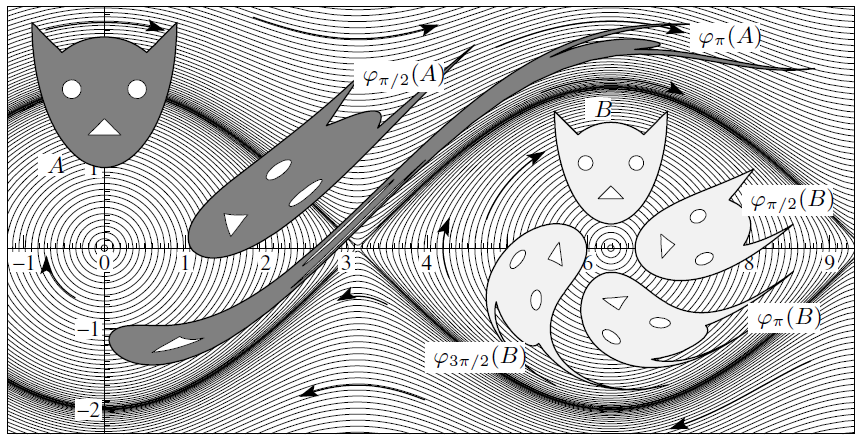
\includegraphics[width=0.75\textwidth]{introduccion/conservacion_volumen_fases.png}
	\caption{Conservación del volumen de fases inicial (representado por el gato) a lo largo de la evolución temporal de un péndulo simple.
	Imagen extraída de \cite[pp. 185]{BOOK:SPR_INT}.}
	\label{fig:cons_gatito}
\end{figure}

\subsubsection{Integradores simplécticos}{\label{sec:int_simpl}}

Dado que la simplecticidad es una propiedad fundamental de todo sistema hamiltoniano, resulta razonable plantear que el integrador que utilicemos para evolucionar temporalmente
el sistema también lo sea.
Decimos que un integrador de un paso es simpléctico si el mapeo asociado $y_1=\Phi_h(y_o)$ es simpléctico.

El primer integrador simpléctico de interés y que usaremos ampliamente es \textit{MidPoint Rule} (MPR), cuyo esquema es
\begin{equation}{\label{eq:MPR}}
 y_{n+1} = y_n + hJ^{-1}\nabla H\left(\frac{y_{n+1}+y_n}{2}\right)
\end{equation}

Veamos que es de orden 2 tomando $y(t_o+h)$ como la solución exacta a \eqref{eq:ec_hamilton} con $y(t_o)=y_o$
\[ y(t_o+h) = y_o + hJ^{-1}\nabla H(y_o) + O(h^2) \]
\begin{align*}
y_1 = y_o + hJ^{-1}\nabla H\left(\frac{y_1+y_o}{2}\right) &=  y_o + hJ^{-1}\nabla H\left(y_o + \frac{h}{2}J^{-1}\nabla H\left(\frac{y_1+y_o}{2}\right)\right) \\
&= y_o + hJ^{-1}\nabla H(y_o) + O(h^2)
\end{align*}
\[ y(t_o+h) - y_1 = O(h^2) \]
por lo que resulta de orden mayor a 1.
Sin embargo, el esquema de MPR es \textit{simétrico} dado que se mantiene al hacer el cambio $y_{n+1}\to y_n$, $y_n\to y_{n+1}$ y $h\to -h$.
Como todo integrador simétrico debe tener orden par, entonces MPR resulta de orden 2 (o superior).

Además, podemos probar que este esquema es simpléctico
\[ \dpart{y_{n+1}}{y_n} = 1 + hJ^{-1}\dpart{}{y_n} \nabla H\left(\frac{y_{n+1}+y_n}{2}\right) = 1 + hJ^{-1} \nabla^2H\left(\frac{y_{n+1}+y_n}{2}\right)\frac{1}{2}\left[ 1+\dpart{y_{n+1}}{y_n} \right]\]
\[ \left[ 1 - \frac{h}{2}J^{-1} \nabla^2H\left(\frac{y_{n+1}+y_n}{2}\right) \right]\dpart{y_{n+1}}{y_n} =  1 + \frac{h}{2}J^{-1} \nabla^2H\left(\frac{y_{n+1}+y_n}{2}\right)\]
donde $1\equiv\mathbb{I}$ la identidad de $\mathbb{R}^{2d}$.
Definiendo $E\equiv\frac{h}{2}J^{-1} \nabla^2H\left(\frac{y_{n+1}+y_n}{2}\right)$ podemos despejar $\dpart{y_{n+1}}{y_n}$
\[ \dpart{y_{n+1}}{y_n} = (1-E)^{-1}(1+E) \]

Buscamos ver que $\left(\dpart{y_{n+1}}{y_n}\right)^TJ\left(\dpart{y_{n+1}}{y_n}\right)= J$, pero antes mostraremos una propiedad útil de $J$ y $E$
\[ E^T J = \frac{h}{2}\left( J^{-1} \nabla^2H \right)^T J = \frac{h}{2} \nabla^2H(J^{-1})^T  J = -\frac{h}{2} \nabla^2H = -JE\]
\[ (1 + E^T)^{-1}J = \sum_{n\geq0} \left(E^T\right)^n J = J\sum_{n\geq0} (-1)^nE^n = J(1 - E)^{-1}  \]

Ahora si podemos probar la simplecticidad de MPR
\begin{align*}
\left(\dpart{y_{n+1}}{y_n}\right)^TJ\left(\dpart{y_{n+1}}{y_n}\right) &= (1+E^T)(1-E^T)^{-1}J(1-E)^{-1}(1+E) \\
&= J(1-E)(1+E)^{-1}(1-E)^{-1}(1+E) = J
\end{align*}


Sin embargo, es inmediato notar que el esquema de MPR no es explícito; no es posible obtener $y_{n+1}$ como una combinación de funciones conocidas aplicadas a $y_n$ para un hamiltoniano $H$ arbitrario.
El integrador puede volverse explícito para hamiltonianos particulares (como el oscilador armónico), pero no lo será en general.

Otro método simpléctico ampliamente utilizado es \textit{Velocity-Verlet} que,a demás de tener el mismo orden resulta explícito para hamiltonianos separables
\[ H(\mathbf{q}_1,..,\mathbf{q}_N,\mathbf{p}_1,..,\mathbf{p}_N) = \sum_i \frac{p_i^2}{2m} + U(\mathbf{q}_1,..,\mathbf{q}_N)\]

El esquema tiene dos versiones, pero la más utilizada es
\begin{align*}
 p_{n+1/2} &= p_n - \frac{h}{2}\dpart{H}{q}(p_{n+1/2}, q_n) \\
 q_{n+1} &= q_n + \frac{h}{2}\left( \dpart{H}{p}(p_{n+1/2}, q_n) + \dpart{H}{p}(p_{n+1/2}, q_{n+1}) \right) \\
 p_{n+1} &= p_{n+1/2} - \frac{h}{2}\dpart{H}{q}(p_{n+1/2}, q_{n+1})
\end{align*}
que para estos hamiltonianos separables resulta explícita
\begin{align*}
 p_{n+1/2} &= p_n - \frac{h}{2}\dpart{U}{q}(q_n) \\
 q_{n+1} &= q_n + \frac{h}{m}p_{n+1/2} \\
 p_{n+1} &= p_{n+1/2} - \frac{h}{2}\dpart{U}{q}(q_{n+1}) = p_n - \frac{h}{2} \left( \dpart{U}{q}(q_n) + \dpart{U}{q}(q_{n+1}) \right)
\end{align*}

Sin embargo, si existe dependencia de momentos en el potencial
\[ H(\mathbf{q}_1,..,\mathbf{q}_N,\mathbf{p}_1,..,\mathbf{p}_N) = \sum_i \frac{p_i^2}{2m} + U(\mathbf{q}_1,..,\mathbf{q}_N;\mathbf{p}_1,..,\mathbf{p}_N)\]
este integrador se vuelve implícito.
Esta es una característica común a todos los integradores simplécticos: solo resultan explícitos para hamiltonianos separables.

Esto resulta muy relevante, dado que implica que el uso de Dinámica Molecular para sistemas interactuantes mediante potencial de Pauli requerirá además la implementación
de algún método para resolver ecuaciones implícitas como \eqref{eq:MPR}.
El costo computacional de estas implementaciones resulta prohibitivo para sistemas de muchas partículas, como mostraremos más adelante.

En la \textbf{Figura \ref{fig:comp_integ_gatito}} podemos ver una comparación de la conservación del volumen de fases para un péndulo simple para los distintos integradores, algunos de los cuales 
compararemos en la sección \ref{sec:choque1D}.

\begin{figure}[H]
	\centering	%trim={<left> <lower> <right> <upper>}
	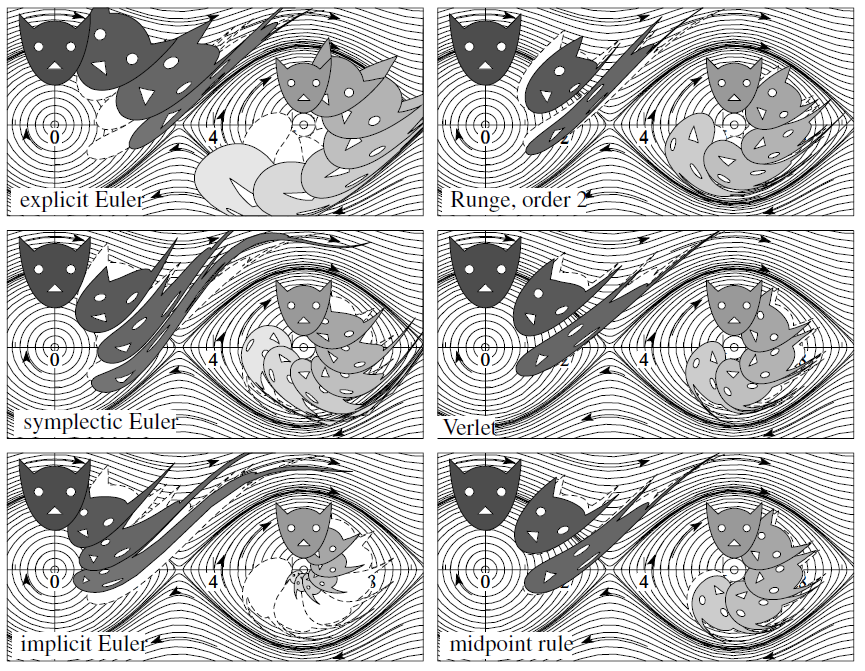
\includegraphics[width=0.9\textwidth]{introduccion/Comparacion_integradores.png}
	\caption{Comparación de la evolución de un dado volumen utilizando distintos integradores (simplécticos o no) para un péndulo ideal.
		Los integradores simplécticos (Verlet, Midpoint Rule y Euler simpléctico) preservan el volumen mejor que los no simplécticos.
		Estas imágenes fueron tomadas de \cite[pp. 188]{BOOK:SPR_INT}}
	\label{fig:comp_integ_gatito}
\end{figure}

\subsection{Método de Metropolis-Montecarlo}

En principio, conocer la función de partición $Z$ otorga acceso a todas las magnitudes termodinámicas de interés.
Para un sistema de $N$ partículas no interactuantes, el hamiltoniano total del sistema puede escribirse como la suma de hamiltonianos de una partícula
\[H(\mathbf{q}_1,..,\mathbf{q}_N;\mathbf{p}_1,..,\mathbf{p}_N) = H_1(\mathbf{q}_1, \mathbf{p}_1) + ... +H_N(\mathbf{q}_N, \mathbf{p}_N)\]
lo cual permite inmediatamente factorizar la función de partición canónica
\[ Z = \int e^{-\beta H(\mathbf{q}_1,..,\mathbf{q}_N;\mathbf{p}_1,..,\mathbf{p}_N)} d^{3N}qd^{3N}p = \prod_{i=1}^N \int e^{-\beta H_i(\mathbf{q};\mathbf{p})} d^{3}qd^{3}p = \prod_{i=1}^N Z_i \]

En general, habrá $n\ll N$ funciones de partición distintas, donde $n$ es la cantidad de tipos de partículas (equivalentemente, la cantidad de hamiltonianos diferentes) y el computo de $Z$ resulta simple.

Para sistemas interactuantes, este método no es aplicable al no ser el hamiltoniano separable; excepto en casos particulares, el cálculo de $Z$ para sistemas interactuantes resulta analíticamente imposible.
Aunque calcular los pesos $e^{-\beta H(\mathbf{q}_1,..,\mathbf{q}_N;\mathbf{p}_1,..,\mathbf{p}_N)}$ para una dada configuración es posible, el cómputo de $Z$ exige barrer el espacio de fases $6N$-dimensional,
cuyo volumen crece exponencialmente con $N$.

Para temperaturas finitas, sin embargo, gran parte de este volumen generará un aporte ínfimo a la función de partición $Z$, al ser estados cuyo peso relativo es bajo.
Por esto mismo, tendrán un aporte ínfimo en los valores medios de las magnitudes termodinámicas de interés.
Por lo tanto, buscamos un método que nos permita evitar por completo el cómputo de $Z$ y tome en cuenta solo las configuraciones relevantes para el sistema a una dada temperatura $T$.
El método de Metropolis-Montecarlo (también conocido como Metropolis-Hastings\cite{Metropolis1953}) nos permite lograr esto mediante el uso de cadenas de Markov.

\subsubsection{Cadenas de Markov}

Las cadenas de Markov son ampliamente utilizadas para modelar múltiples fenómenos (biológicos, económicos, sociales) por su simplicidad y teoría bien desarrollada\cite[pp. 1]{BOOK:DURRET}.
El objetivo de las cadenas de Markov es introducir la memoria en una sucesión de variables aleatorias $(X_n)_{n\in \mathbb{N}}$ de la forma más simple posible.
Esto es, la evolución $X_n \to X_{n+1}$ no depende de los $n-1$ estados previos ni del ``tiempo'' $n$, sino únicamente del estado actual $X_n$.

Con esto en mente, una sucesión de variables aleatorias $(X_n)_{n\in \mathbb{N}}$ es una cadena de Markov a tiempo discreto si
\[ P(X_{n+1}=j | X_n = i, X_{n-1} = i_{n-1}, ..., X_o = i_0) = P(X_{n+1}=j | X_n = i)  \]
donde $j, i, i_{n-1}, ..., i_0$ son estados posibles de la cadena.

Se define la matriz de transición $p(i,j)$ de la cadena de Markov como la probabilidad de alcanzar el estado $j$ partiendo del estado $i$, aprovechando la independencia del tiempo $n$
\[ p(i,j) = P(X_{n+1} = j | X_n = i) \]

En particular, si nos interesa ver las probabilidades de transición múltiples pasos adelante (a $n$ pasos)
\begin{align*}
 p_n(i,j) = P(X_n = j | X_0 = i) &= \frac{P(X_n = j, X_0 = i)}{P(X_0 = i)} \\
 &= \sum_k \frac{P(X_n = j, X_{n-1}=k, X_0 = i)}{P(X_0 = i)} \\
 &= \sum_k P(X_n = j| X_{n-1}=k, X_0 = i)\frac{P(X_{n-1}=k, X_0 = i)}{P(X_0 = i)} \\
 &= \sum_k P(X_n = j| X_{n-1}=k)P(X_{n-1}=k| X_0 = i) \\
 &= \sum_k p(k,j)p_{n-1}(i,k)
\end{align*}

Identificando la suma anterior como el producto de matrices $(p_{n-1} \cdot p)(i,j)$ y usando que $p_1(i,j)=p(i,j)$, resulta inmediato que $p_n(i,j) = p^n(i,j)$.
En esta propiedad reside la simplicidad de las cadenas de Markov.

En particular, nos interesan las cadenas de Markov irreducibles; aquellas en las que todo estado $i$ puede alcanzar el estado $j$ en una cantidad finita de pasos.
Matemáticamente, decimos que una cadena de Markov es irreducible si
\[ \forall i,j \quad \exists n\in \mathbb{N} \text{ tal que } p^n(i,j) \neq 0 \]

El caso más simple de una cadena no irreducible es una con dos conjuntos de estados $A$ y $B$ desconectados entre si.
\[ p =
\begin{pmatrix}
 p_A & 0\\
 0 & p_B
\end{pmatrix} \]
En estos casos, resultaría mucho más sensato tratarla como dos cadenas de Markov de estados $A$ y $B$ con sus respectivas matrices $p_A$ y $p_B$.

El otro caso de cadena no irreducible es aquella con estados absorbentes\cite[pp. 6]{BOOK:DURRET}; aquellos que no pueden transicionar a otros estados.
Decimos que un estado $i$ es absorbente si $p(i,j)=\delta_{ij} \text{ } \forall j$.
Estas cadenas, en principio, pueden utilizarse para modelar ciertos problemas como la ``Ruina del jugador''\cite[pp. 1]{BOOK:DURRET}. 
Este problema representa a un apostador que jugará hasta quedarse sin dinero o ganar un dinero $N$ total.
Cada vez que apuesta, tiene una probabilidad $p$ de ganar 1 y una probabilidad $1-p$ de perder 1, tal que
\[ p(i,j) = \delta_{j,i+1}p+\delta_{j,i-1}(1-p) \qquad 0<i<N \]
\[ p(i,j) = \delta_{i,j} \qquad i=0,N \]
donde claramente los estados $0$ y $N$ son absorbentes.

En el método de Montecarlo, las cadenas de Markov utilizadas son irreducibles dado que tienen lo que se conoce como una \textit{distribución estacionaria}, que describimos a continuación.

\subsubsection{Distribución estacionaria}

Cuando el estado inicial de una cadena de Markov tiene una distribución $q(i)$, podemos usar el resultado anterior para calcular la distribución $n$ pasos después
\[ P(X_n=j) = \sum_i P(X_n=j,X_0=i) =  \sum_i P(X_n=j|X_0=i)P(X_0=i) = \sum_i p^n(i,j)q(i) = (q\cdot p^n)(j)\]
usando el producto habitual de matrices y tomando el vector fila de probabilidades $q$.
Por lo tanto, la distribución de probabilidad a tiempo $n$ se relaciona con la inicial según $q_n = q_0\cdot p^n$ o, recursivamente, $q_{n+1} = q_n\cdot p$.

Resulta natural entonces preguntarse si existirá alguna forma de mantener la distribución constante $q_{n+1} = q_n$.
Esto es equivalente a pedir que $q_n$ sea un autovector de $p$ con autovalor 1.
Para diferenciar, llamaremos $\pi(x)$ a esta distribución estacionaria que cumple $\pi p = \pi$.

Obtener $\pi$ implica resolver las \textit{ecuaciones de balance}
\[ \sum_k \pi(k) p(k, j) = \pi(j) \]

Sin embargo, muchas veces resulta más natural el uso de las \textit{condiciones de balance detallado}
\[ \pi(k) p(k, j) = \pi(j)p(j, k) \qquad \forall j,k \]
que nos arroja inmediatamente las ecuaciones de balance al sumar sobre $k$.
\[ \sum_k \pi(k) p(k, j) = \sum_k \pi(j)p(j, k) = \pi(j) \sum_k p(j,k) = \pi(j) \]

Claramente, la condición de balance detallado resulta más fuerte que la de balance y no necesariamente puede cumplirse.
Sin embargo, cuando existe, puede ser mucho más sencilla de encontrar.
Esto es particularmente cierto para el caso de matrices de transición $p$ ralas (con gran cantidad de ceros), donde las condiciones de balance detallado se simplifican (como en la ``Ruina del jugador'' explicada previamente).

A continuación, enunciaremos dos teoremas relevantes para el método de Metropolis\cite[pp. 26]{BOOK:DURRET}.
El primero asegura la existencia de una única distribución estacionaria como solución a las ecuaciones de balance (pero no necesariamente balance detallado).

\begin{theorem}
 Sea $p$ una matriz de transición finita e irreducible. Luego, existe solución única a las ecuaciones de balance $\pi p = \pi$ con $\sum_k \pi(k) = 1$ y $\pi(k)\geq 0$ $\forall k$
\end{theorem}

Es importante aclarar que la hipótesis de matriz finita es necesaria para poder asegurar la normalización de $\pi$.
Existe una versión del teorema para dimensión infinita, pero no es relevante para nuestro tratamiento actual, donde nos limitaremos a un conjunto de estados finito.
Volveremos sobre esto más adelante.

Pero la existencia de una distribución estacionaria puede no ser suficiente si somos incapaces de calcularla.
Si la cadena de Markov comienza con una distribución inicial $q(i)$ cualquiera, esperaríamos que eventualmente alcance la distribución estacionaria.
El siguiente teorema es análogo a la Ley de los Grandes Números para el caso de cadenas de Markov y nos asegura lo anterior, entre otras cosas.

\begin{theorem}{\label{teo:markov_muestreo}}
 Sea $p$ una matriz de transición irreducible con distribución estacionaria $\pi$ y $f$ una función sobre los estados tal que $\sum_x f(x)\pi(x) < \infty$, entonces
 \[ \lim_{n\to\infty} \frac{1}{n} \sum_{m=1}^n f(X_m) = \sum_x f(x)\pi(x) \]
\end{theorem}

Para obtener la convergencia, basta tomar la función $f(x) = \delta_{xy}$ para algún $y$, de forma tal que $\sum_{m=1}^n f(X_m)$ sea la cantidad de tiempo que el sistema estuvo en $y$.
Por el teorema anterior, esto converge a $\pi(y)$.
Pero este teorema es más general y nos permite obtener distintos observables $f$ de la distribución, propiedad que nos resultará muy útil cuando apliquemos el algoritmo.


\subsubsection{Algoritmo de Metropolis-Montecarlo}{\label{sec:alg_mm}}

El objetivo de este algoritmo es obtener muestras de una dada distribución $\pi$ construyendo una cadena de Markov que la tenga como distribución estacionaria.
Para esto, fabricaremos una matriz de transición $p$ que cumpla las condiciones de balance detallado con $\pi$.

Comenzamos con una cadena de Markov con matriz $q(x,y)$ representando la transición propuesta.
Sin embargo, aceptaremos la transición con probabilidad\cite{Metropolis1953}
\[r(x,y) = \min \left\{ \frac{\pi(y)q(y,x)}{\pi(x)q(x,y)}, 1\right\}\]
de forma tal que la probabilidad de transición final resulta $p(x,y) = q(x,y)r(x,y)$.

Veamos que esta $p$ cumple las ecuaciones de balance detallado.
Supongamos $\pi(y)q(y,x) \leq \pi(x)q(x,y)$ tal que 
\[
r(x,y) = \pi(y)q(y,x)/\pi(x)q(x,y) \quad \text{y} \quad r(y,x) = 1\]
\[ \pi(x) p(x, y) = \pi(x) q(x,y)\frac{\pi(y)q(y,x)}{\pi(x)q(x,y)} = \pi(y)q(y,x) = \pi(y)q(y,x)r(y,x) = \pi(y)p(y,x) \]
El caso opuesto resulta completamente análogo.

Para generar muestras con distribución $p$, basta evolucionar temporalmente la cadena durante un tiempo suficientemente largo hasta que alcance el equilibrio y
aprovechar el teorema \ref{teo:markov_muestreo} para muestrear los valores medios de las magnitudes termodinámicas de interés.

En nuestro caso, tomamos los estados $x = (\mathbf{q}_1,..,\mathbf{q}_N;\mathbf{p}_1,..,\mathbf{p}_N)$ como distintas configuraciones del espacio de fases.
Queremos como distribución estacionaria la predicha por el ensamble canónico \[\pi(x) = \frac{e^{-\beta E_x}}{Z} = \frac{1}{Z}e^{-\beta H(\mathbf{q}_1,..,\mathbf{q}_N;\mathbf{p}_1,..,\mathbf{p}_N)}\]
Como dijimos, este algoritmo nos ahorra el problema de calcular la función de partición $Z$, dado que las probabilidades de transición $p$ dependen del cociente de los $\pi(x)$.

Sin embargo, el espacio de fases $6N$-dimensional es continuo y, por lo tanto, la cantidad de estados $x$ es infinita.
Esto no es particularmente problemático dado que toda simulación computacional fuerza el problema a ser finito.
Por lo tanto, el espacio de fases pasa a ser una red finita $6N$-dimensional y podemos usar todo el aparato anterior.

Podemos elegir esta matriz de transición proponiendo pasos en los que seleccionamos una partícula $i$ con probabilidad $1/N$, moviendo sus coordenadas canónicas a otras dentro de un paralelepípedo
centrado en su valor actual
\[
\left\{\begin{matrix}
\mathbf{q}_i \to  \mathbf{q}_i + \Delta_q \mathbf{a} & & a_k,b_k \text{ variables aleatorias independientes y }  \\
\mathbf{p}_i \to  \mathbf{p}_i + \Delta_p \mathbf{b} & &  \text{uniformes en } \{2\frac{j}{M}-1: j\in\mathbb{Z}, 0 \leq j \leq M\}
\end{matrix}\right.\]
donde $M$ es un entero (suele ser el máximo representable por un \texttt{long int} $M = 2^{31}-1\sim 10^9$).

Por lo tanto, si $x$ e $y$ difieren en las coordenadas de más de una partícula tenemos $q(x,y)=0$.
Si difieren unicamente en las coordenadas de la partícula $i$, tenemos
\[q(x,y) = \frac{\Theta(\Delta_q - \Arrowvert \mathbf{q}_i - \mathbf{q}_i' \Arrowvert_\infty)\Theta(\Delta_p - \Arrowvert \mathbf{p}_i - \mathbf{p}_i' \Arrowvert_\infty)}{N(2M+1)^6}\]
por lo que nuestra elección de $q$ es simétrica con $q(x,y) = q(y,x)$.

Aprovechando la simetría de $q$, la probabilidad de aceptación se simplifica
\[r(x,y) = \min\left\{\frac{\pi(y)}{\pi(x)}, 1\right\} = \min\{e^{-\beta(E_y-E_x)}, 1\}\]
De esta forma, si tenemos que $\Delta E = E_y - E_x \leq 0$ aceptamos inmediatamente. Si resulta $\Delta E > 0$, aceptamos con probabilidad $e^{-\beta\Delta E}$.


\subsection{Teorema $\Pi$ y adimensionalización}{\label{sec:intro_pi}}

Es interesante que podamos explotar la independencia de las leyes naturales respecto del sistema de unidades elegido, pues nos dice que toda relación física puede expresarse en forma adimensional. 
Esta propiedad nos permite realizar un \textit{análisis dimensional} para simplificar problemas, proponer leyes de \textit{scaling} e interpretar resultados experimentales.

En esta formulación, usamos que toda ley física puede expresarse en función de sus parámetros $a_1,...,a_n$ como una curva de nivel
\[ f(a_1,...,a_n) = 0 \]

El teorema de Buckingham\cite[pp. 21-22]{BOOK:KUNDU} (también conocido como teorema $\Pi$) dice que las $n$ variables siempre pueden combinarse para formar 
$(n-r)$ variables adimensionales, donde $r$ es la cantidad de dimensiones del problema. 
De esta manera, podemos reescribir la relación anterior como
\begin{equation}{\label{eq:teo_pi}}
\Phi(\Pi_1,..,\Pi_{n-r}) = 0 \qquad \text{ o } \qquad \Pi_1=\phi(\Pi_2,..,\Pi_{n-r})
\end{equation}

Para problemas de mecánica, suele ser $r=3$ en correspondencia con las 3 unidades fundamentales: masa $M$, distancia $L$ y tiempo $T$.
Si agregamos la termodinámica, se suma la temperatura $\theta$, generalmente acompañada de la constante de Boltzmann $k_B$.
Es por esto que es muy habitual trabajar directamente con la magnitud $k_BT$, cuyas unidades son de energía y pueden relacionarse con las de la mecánica $[k_BT] = ML^2/T^2$.

Es por eso que en general, en las simulaciones de mecánica estadística solemos tomar directamente $k_B=1$ (medimos la temperatura en unidades de energía) y tenemos $r=3$.
Esto significa que no necesitamos analizar las $n$ variables del sistema, sino las $n-3$ variables adimensionales, lo cual es muy valioso al permitirnos acotar el espacio de búsqueda.
Esto es especialmente cierto para $n<10$, donde la reducción de la cantidad de variables en 3 resulta apreciable.
Sistemas con una cantidad $n$ de parámetros muy grande no permiten un muestreo completo de todas las variables, sean $n$ o $n-r$.

Un claro ejemplo de la aplicación de este teorema en mecánica estadística es el caso de un gas de partículas interactuando vía el potencial de Lennard-Jones (LJ)
\[ V_{LJ}(r) = \varepsilon\left( \left( \frac{\sigma}{r} \right)^{12} - \left( \frac{\sigma}{r} \right)^6 \right) \]
cuyo hamiltoniano dependerá de la masa $m$ además de los 2 parámetros de Lennard-Jones $\varepsilon$ y $\sigma$.
Además, tenemos las 2 variables termodinámicas a elección, como por ejemplo la densidad $\rho$ y la temperatura $T$.
Por lo tanto, tenemos 5 parámetros del sistema y 3 unidades, por lo que las variables adimensionales de interés bien pueden ser $T^* = T/\varepsilon$ y $\rho^*=\rho\sigma^3$. 
Estas serán las variables que rigen el comportamiento termodinámico del sistema.
También podemos construir $r^*=r/\sigma$, $p^*=p/\sqrt{m\varepsilon}$ y así con todas las magnitudes de interés.

Esto resulta equivalente a pensar que en lugar de usar metro-kilo-segundo (mks), estamos usando $\sigma - m - \sqrt{\varepsilon/m\sigma^2}$.
En este sistema de unidades, tenemos básicamente $\sigma=1=m=\varepsilon$, lo cual también suele llamarse \textit{unidades reducidas}.
A efectos prácticos, estamos \textit{eliminando} las variables $\sigma,m,\varepsilon$ de nuestro análisis.
Luego, todos los gases de LJ con $\sigma$ y $\varepsilon$ a densidad $\rho$ y temperatura $T$ son equivalentes a un LJ con $\sigma=1=\varepsilon=m$ y
densidad $\rho\sigma^3$ y temperatura $T/\varepsilon$; cambiar los parámetros equivale a reescalar las variables termodinámicas.

Como dijimos esto es una cuestión semántica dado que ambos abordajes son equivalentes y facilitan mucho el análisis de las formas funcionales de las distintas relaciones entre parámetros.
Esto será particularmente útil en las secciones \ref{sec:choque1D} y \ref{sec:pauli_gas}, donde veremos que la cantidad de parámetros involucrados en el análisis es comparable a $r$.


\subsection{Función de distribución radial}{\label{sec:intro_gr}}

En el estudio del potencial de Pauli, resulta interesante analizar si pueden existir fases no gaseosas de un sistema interactuando mediante este potencial.
Sin embargo, las simulaciones vía el algoritmo de Metropolis-Montecarlo tiene una inherente dificultad para muestrear observables asociados a la evolución temporal del sistema.
Esto hace que algunos indicadores como el \textit{coeficiente de Lindemann} resulten difíciles de interpretar a la hora de observar transiciones de fase.
Esto ocurre porque este coeficiente mide las fluctuaciones en la posición de las partículas como una forma de analizar su desplazamiento, lo cual carece de sentido para una simulación de Montecarlo.

Sin embargo, la función de distribución radial $g(r)$ cuantifica la cantidad de pares de partículas a distancia $r$, lo cual es fácilmente obtenible en una simulación de Montecarlo.
Esta función de distribución radial se define según 
\begin{equation}{\label{eq:def_gr}}
 g(r) = \frac{2}{N}\frac{\left< N(r,\Delta r) \right>}{\rho V(r,\Delta r)} \approx \frac{2}{N}\frac{\left< N(r,\Delta r) \right>}{\rho 4\pi  r^2\Delta r}
\end{equation}
donde $N(r,\Delta r)$ es la cantidad de partículas dentro de un cascarón esférico de radio $r$ y grosor $\Delta r$ centrado en otra partícula y $V(r,\Delta r)$ es el volumen de dicho cascarón\cite{BOOK:HAILE}.
La aproximación vale para $\Delta r$ pequeño, lo cual es ciertamente deseable para tener una discretización fina.

Para un sistema gaseoso, esperamos que $g(r)$ tienda a 1 rápidamente, dado que el sistema es caótico y tiende a tener partículas a todas las distancias.
En contraposición, un sistema sólido tendrá un $g(r)$ compuesta por picos en distancias características dependientes de la estructura de la red.
Un sistema líquido tendrá una $g(r)$ intermedia, con ciertas oscilaciones alrededor de 1.
En los 3 casos, debemos tener $g(r)\to 1$ para $r$ suficientemente grande y, para potenciales de núcleo duro, esperamos una $g(r)=0$ para $r\leq r_o$ ($r_o$ es el ``radio'' de cada partícula).
En la \textbf{Figura \ref{fig:gr_fases}} podemos ver estos casos para un gas de Lennard-Jones.

\begin{figure}[H]
	\centering	%trim={<left> <lower> <right> <upper>}
	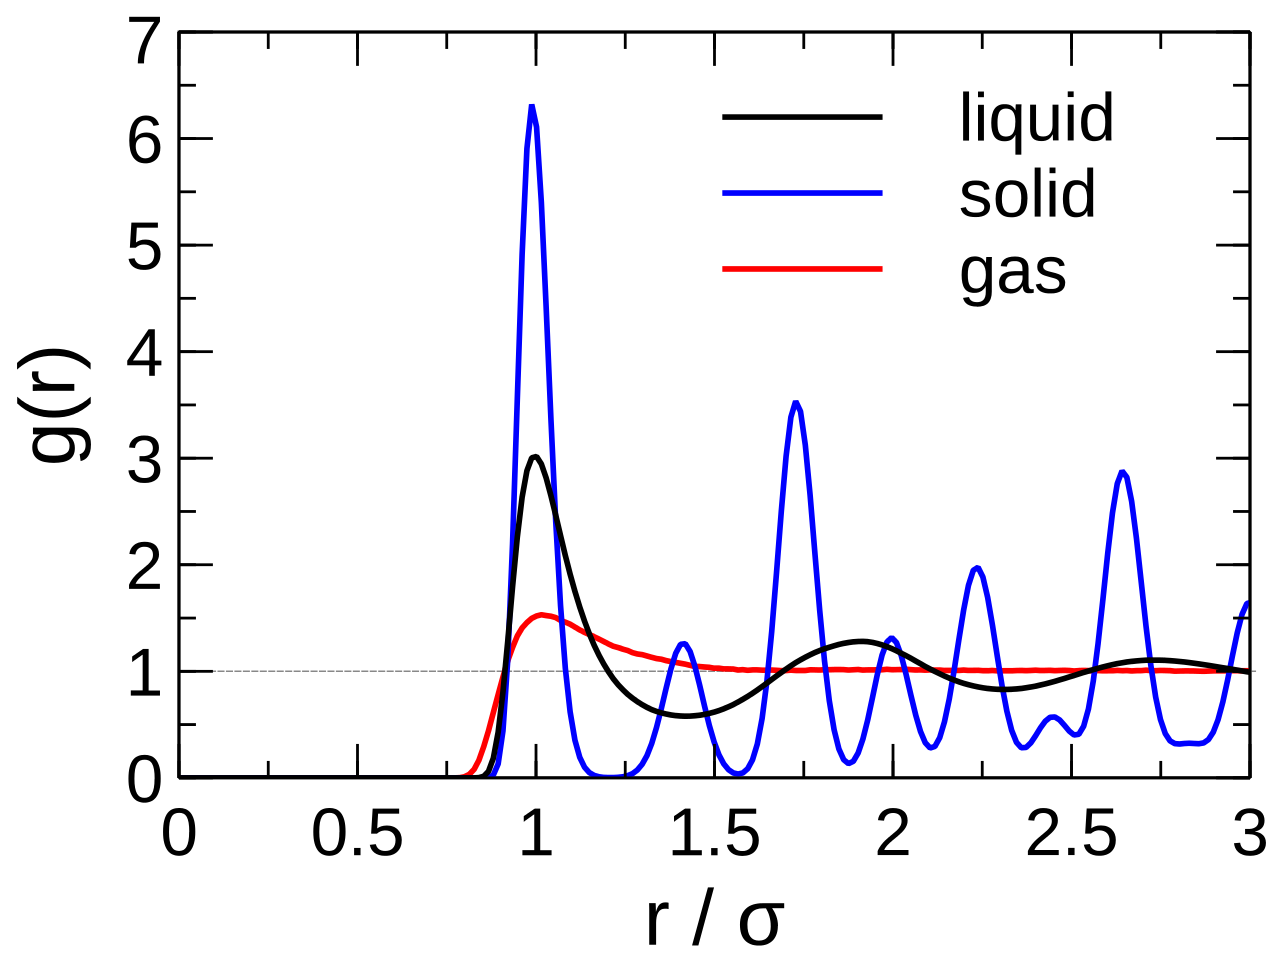
\includegraphics[width=0.5\textwidth]{introduccion/gr_fases.png}
	\caption{Función de distribución radial para las distintas fases de un gas de Lennard-Jones}
	\label{fig:gr_fases}
\end{figure}

\subsection{Materia Nuclear}{\label{sec:intro_NM}}

La Materia Nuclear (NM) consiste en un sistema termodinámico de nucleones eléctricamente neutros, interactuando unicamente mediante interacción nuclear (sin Coulomb)\cite{Molinelli}.
En general, cuantificamos mediante $\delta=(N_n - N_p)/N$ la asimetría entre la cantidad neutrones $N_n$ y protones $N_p$.
Para $\delta=0$, decimos que el sistema es \textit{simétrico}.
Este parámetro se suma a los habituales $T$ y $\rho$ a la hora de obtener una ecuación de estado $U(T,\rho, \delta)$.

Ciertamente, no debe confundirse NM con los nucleones de los átomos.
La formulación de NM asume sistemas infinitos, extensivos y neutros muy diferentes a los núcleos atómicos.
Esta cuestión dificulta la vinculación directa de los resultados teóricos con los obtenidos experimentalmente.

En el abordaje clásico del problema, se modela la interacción nuclear como un potencial efectivo.
Existen múltiples formulaciones de este potencial, pero aquí nos concentraremos en el conocido como QCNM\cite{Dorso1988} (\textit{Quasi-Classical Nuclear Matter}), cuyo potencial de interacción entre \textit{todos los nucleones} es

\begin{equation}{\label{eq:pot_QCNM}}
 V_N(r) = V_o \left[ \left(\frac{r_1}{r}\right)^{p_1} - \left(\frac{r_2}{r}\right)^{p_2} \right] \left( 1 + e^{\frac{r-d}{a}} \right)^{-1}
\end{equation}

Este potencial fue inspirado por el potencial de Lennard-Jonnes, que resulta atractivo a distancia finita y repulsivo a corta distancia, como se espera de la interacción nuclear.
Sin embargo, para corregir el alcance de este potencial se introdujo un decaimiento exponencial.
La intensidad del potencial se tomó $V_o=25.93$MeV con potencias $p_1=6.2$ y $p_2=3.0$, distancias características $r_1=1.757$fm y $r_2=1.771$fm y modulación exponencial $d=3.35$fm y $a=0.833$fm.
De esta manera, hay un mínimo de potencial en $r\approx 2.138$fm de $-5.722$MeV, como puede apreciarse en la \textbf{Figura \ref{fig:graf_QCNM}}.

\begin{figure}[H]
	\centering
	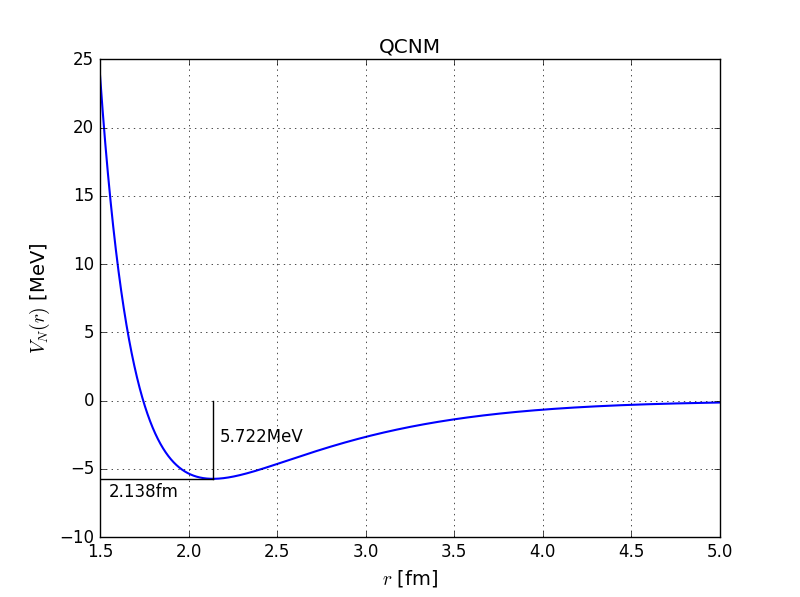
\includegraphics[width=0.7\columnwidth]{introduccion/QCNM_pot.png}
	\caption{Parametrización QCNM del potencial nuclear. 
	El mínimo de potencial se encuentra a $r_o=2.138$fm con $V_N(r_o)=-5.722$MeV.}
	\label{fig:graf_QCNM}
\end{figure}

El hecho de que este potencial trate de forma idéntica protones y neutrones no es una característica general.
Existen potenciales como el CMD que separan la interacción entre $V_{np}$ y $V_{nn/pp}$ donde la interacción entre nucleones idénticos es puramente repulsiva mientras que la interacción protón-neutrón 
es atractiva a distancia finita y repulsiva a distancias cortas.

En general, los parámetros de todos estos potenciales se ajustan para que la energía y la densidad de saturación coincidan con los valores experimentales $E_{NM}^{sat}=-16$MeV y $\rho_o=0.16$fm$^{-3}$\cite{Dorso1988}.
Estas curvas de energía $E(\rho)$ suelen ser cóncavas, con un único mínimo claro.
Trabajos recientes \cite{Schrader2009,GimenezMolinelli2014, GimenezMolinelli2015} han mostrado que para densidades debajo de la densidad de saturación, la curva pierde su concavidad y el sistema entra en un 
régimen de \textit{pastas nucleares}; configuraciones no homogéneas de las partículas.
En este régimen de pastas, la curva se vuelve cuasi-constante, oscilando alrededor de un valor aproximado $-13$MeV (en $T=0.5$MeV)\cite{Dorso2018}; todas las pastas disponen de la misma energía de ligadura (ver \textbf{Figura \ref{fig:curva_Evsrho_dorso}}).

\begin{figure}[H]
	\centering
	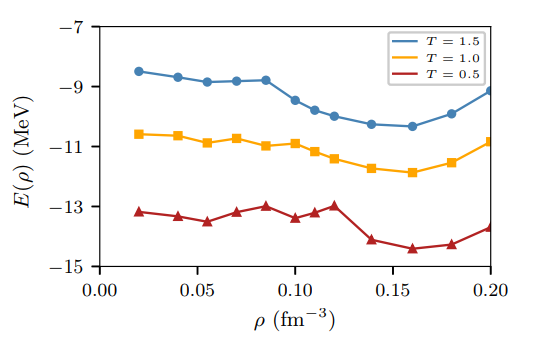
\includegraphics[width=0.6\columnwidth]{introduccion/curva_Evsrho_dorso.png}
	\caption{Energía por nucleón en función de densidad para las simulaciones de materia nuclear de \cite{Dorso2018}.
	En el régimen de pastas para $\rho\leq\rho_o$ la energía se vuelve constante, oscilando alrededor de un valor fijo.}
	\label{fig:curva_Evsrho_dorso}
\end{figure}

Estas estructuras se observan principalmente en simulaciones de \textit{Neutron Star Matter} (NSM), donde se sabe que surgen de la competencia entre interacciones nucleares (como CMD o QCNM) e interacción de Coulomb. 
Para sistemas con interacción nuclear sin Coulomb, sin embargo, se sospecha que pueden deberse a efectos de tamaño finito y/o a las condiciones de contorno periódicas.

En contraposición a NSM, las pastas halladas en NM suelen disponer de una única estructura por celda.
Es por todo esto que habitualmente de las denomina \textit{pseudo-pastas}.
Generalmente, las pastas surgidas de estos potenciales clásicos suelen tener una fase líquida seguida de una fase sólida-cristalina a temperatura baja \cite{Dorso2018,Alcain,Dorso2019}.